\chapter{A/B 测试实验}
\label{chap:ab-test}

本章面向真实 WebRTC 端到端链路，给出离线强化学习策略与浏览器默认 GCC 拥塞控制算法的 A/B 对比实验设计、测试过程与结果分析。实验目标并非在所有网络条件下单纯追求更高吞吐，而是验证本文在第五章给出的 IQL 策略在真实链路中能否以较低的部署风险换取更稳定、更低时延、更低丢包且动作更平滑的整体 QoE 表现，并进一步讨论策略在不同网络场景下的适用边界。

\section{实验目标与对比策略}

本研究将浏览器端默认启用的 Google Congestion Control（GCC）作为对照策略（Control），将基于离线强化学习训练得到的 IQL Actor 策略作为实验策略（Treatment）。两者的核心差异在于：GCC 通过接收端延迟梯度与丢包反馈的启发式规则调整估计带宽，而离线强化学习策略在每个控制周期根据状态窗口（发送/接收吞吐、RTT、抖动、丢包率等）直接输出带宽上限动作，并通过 \texttt{RTCRtpSender.setParameters()} 将其施加为 \texttt{maxBitrate}，从而形成“策略输出 → 发送端限速 → 网络反馈 → 下一步决策”的闭环。

为避免推理链路与媒体流共享同一网络信道导致控制滞后（第五章已讨论），A/B 测试默认采用浏览器端 ONNX 本地推理：策略模型以 \texttt{actor.onnx} 形式加载至页面侧并用 \texttt{onnxruntime-web} 执行推理，从而将控制链路与网络环境扰动解耦。

在实验策略的模型工件选择上，为降低在线对比的试错成本，本研究采用离线验证集上的 \textbf{NLL 最优} 作为 checkpoint 选择准则：在训练过程中每 5,000 步计算一次验证集 NLL，并选取 NLL 达到最小值时对应的 \texttt{checkpoint\_50000}。随后将该 checkpoint 中的 \texttt{actor.pt} 导出为 \texttt{actor.onnx}，作为 A/B 测试阶段 RL 实验组的部署模型，与 GCC 对照组在相同网络场景下进行对比。该做法的动机在于，高斯策略网络的训练目标与验证指标均以对数似然为核心，NLL 更能一致地反映策略对离线数据分布的拟合质量；在缺乏在线探索的前提下，优先使用 NLL 最优的 checkpoint 有助于在上线验证中获得更稳定、可解释的策略行为。

\section{网络场景}

A/B 测试阶段完全复用第四章 4.1.2 中定义的九类网络环境及其 \texttt{pfctl + dummynet} 参数配置。

\begin{figure}[htbp]
    \centering
    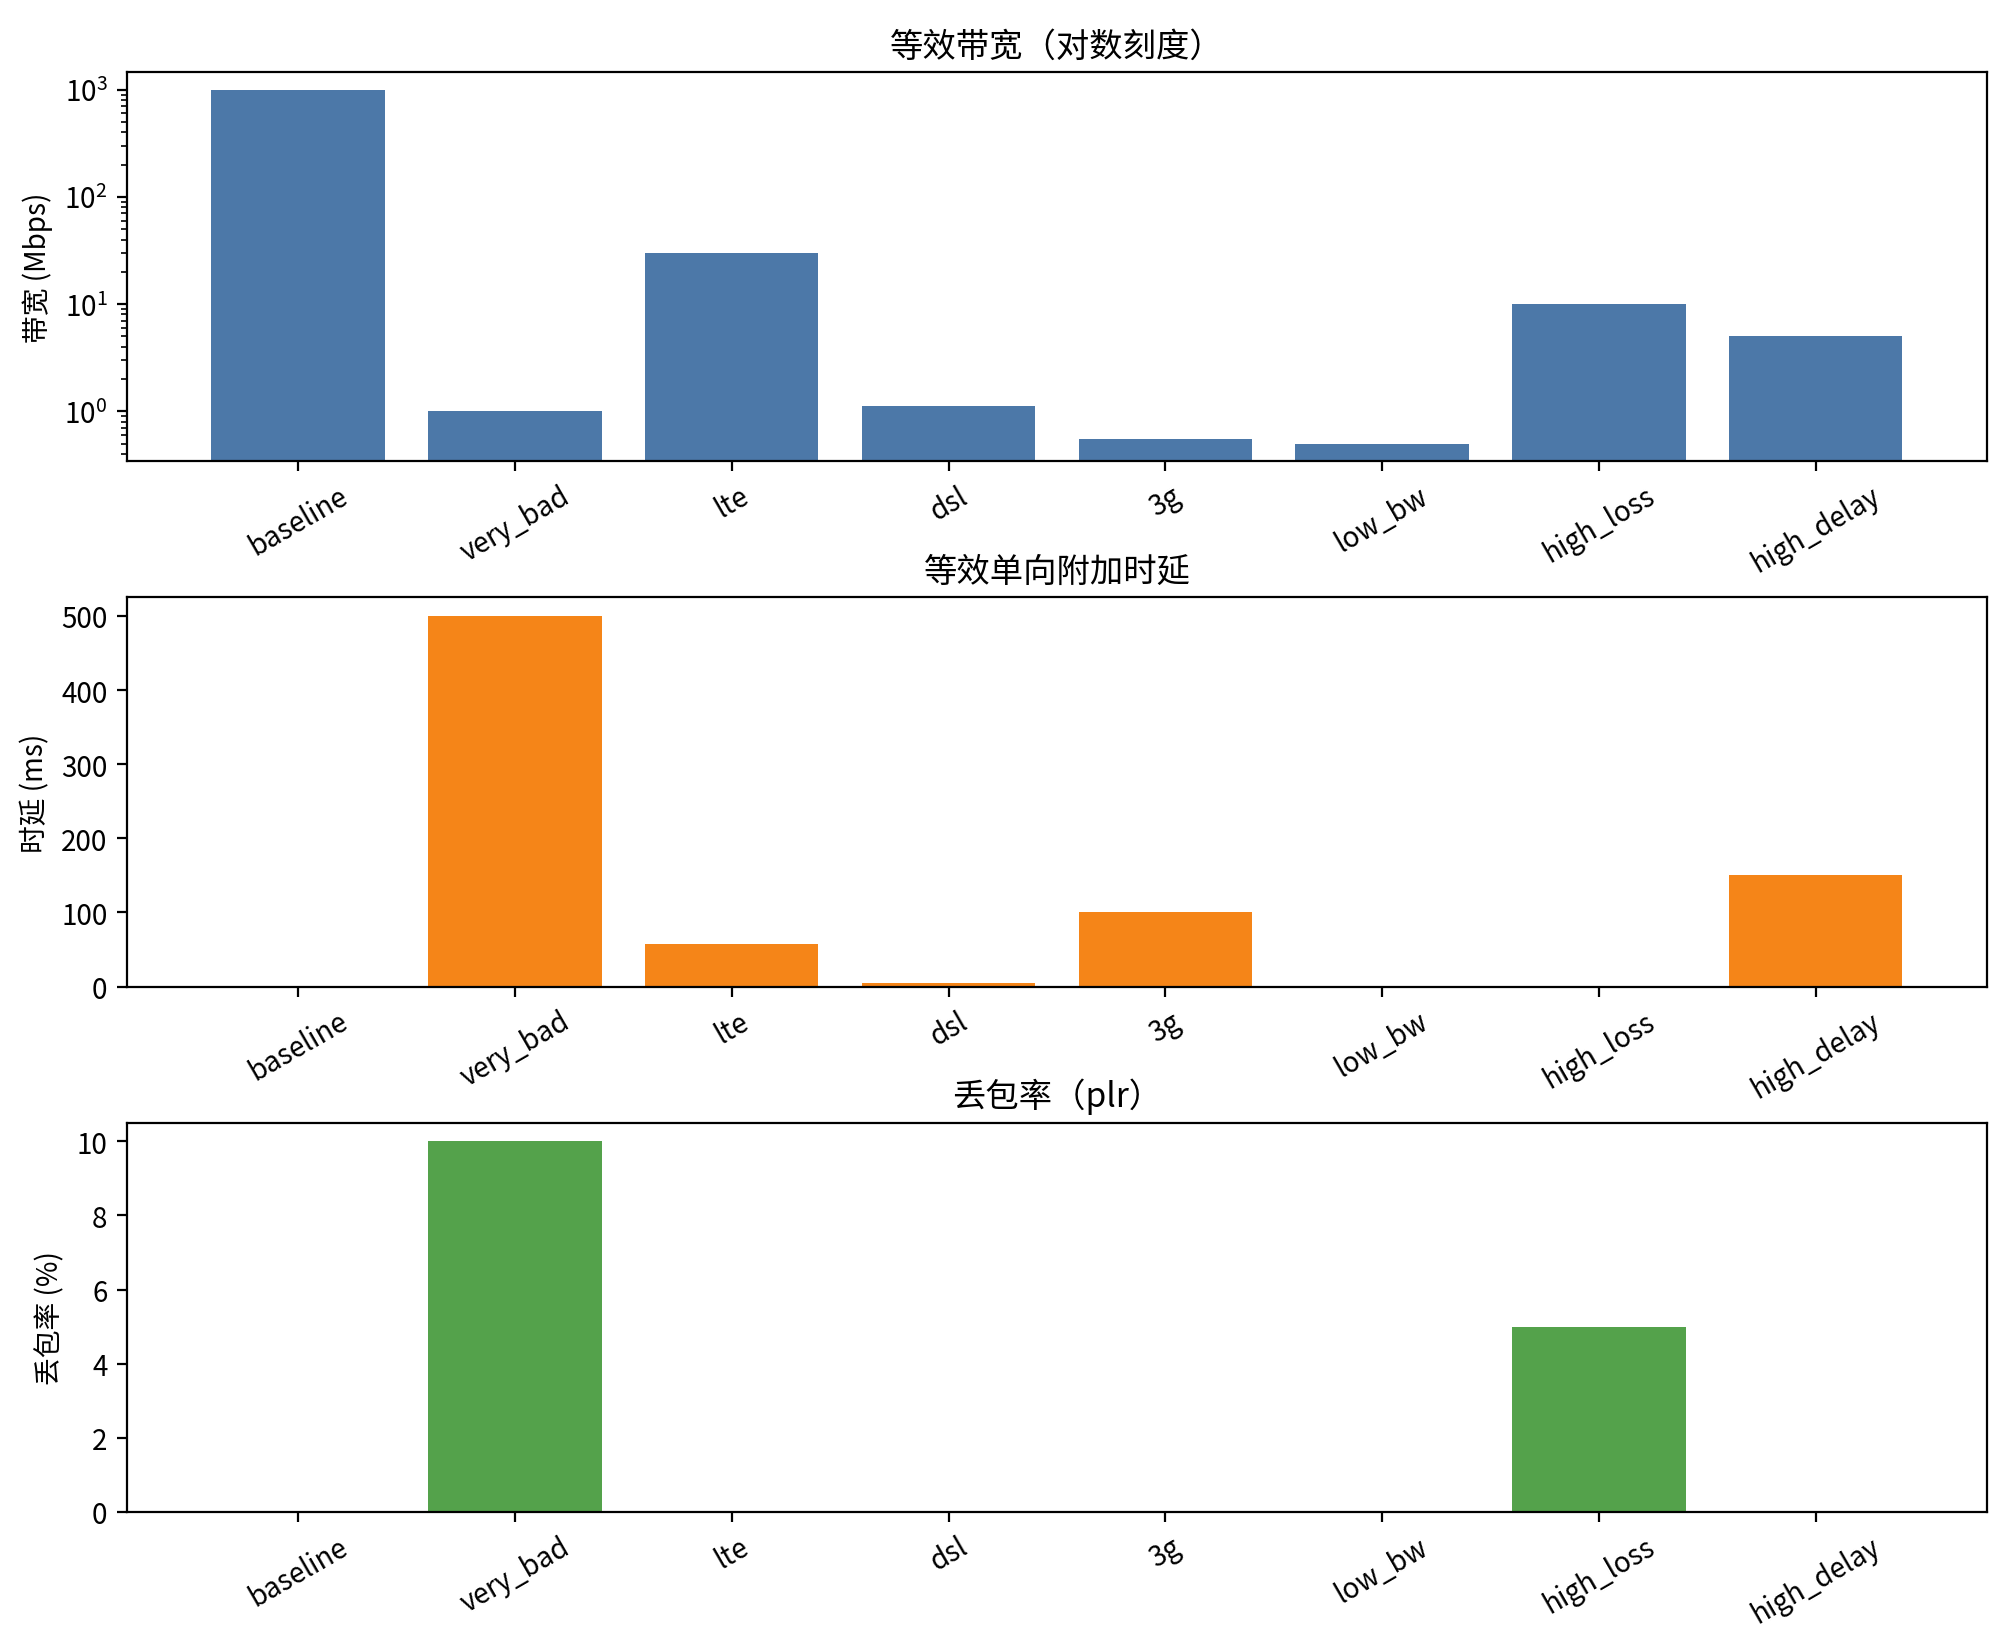
\includegraphics[width=0.95\textwidth]{figures/chapter6/network_condition_parameter.png}
    \caption{网络场景参数总览（静态场景）}
    \label{fig:network-condition-parameter}
\end{figure}

\begin{figure}[htbp]
    \centering
    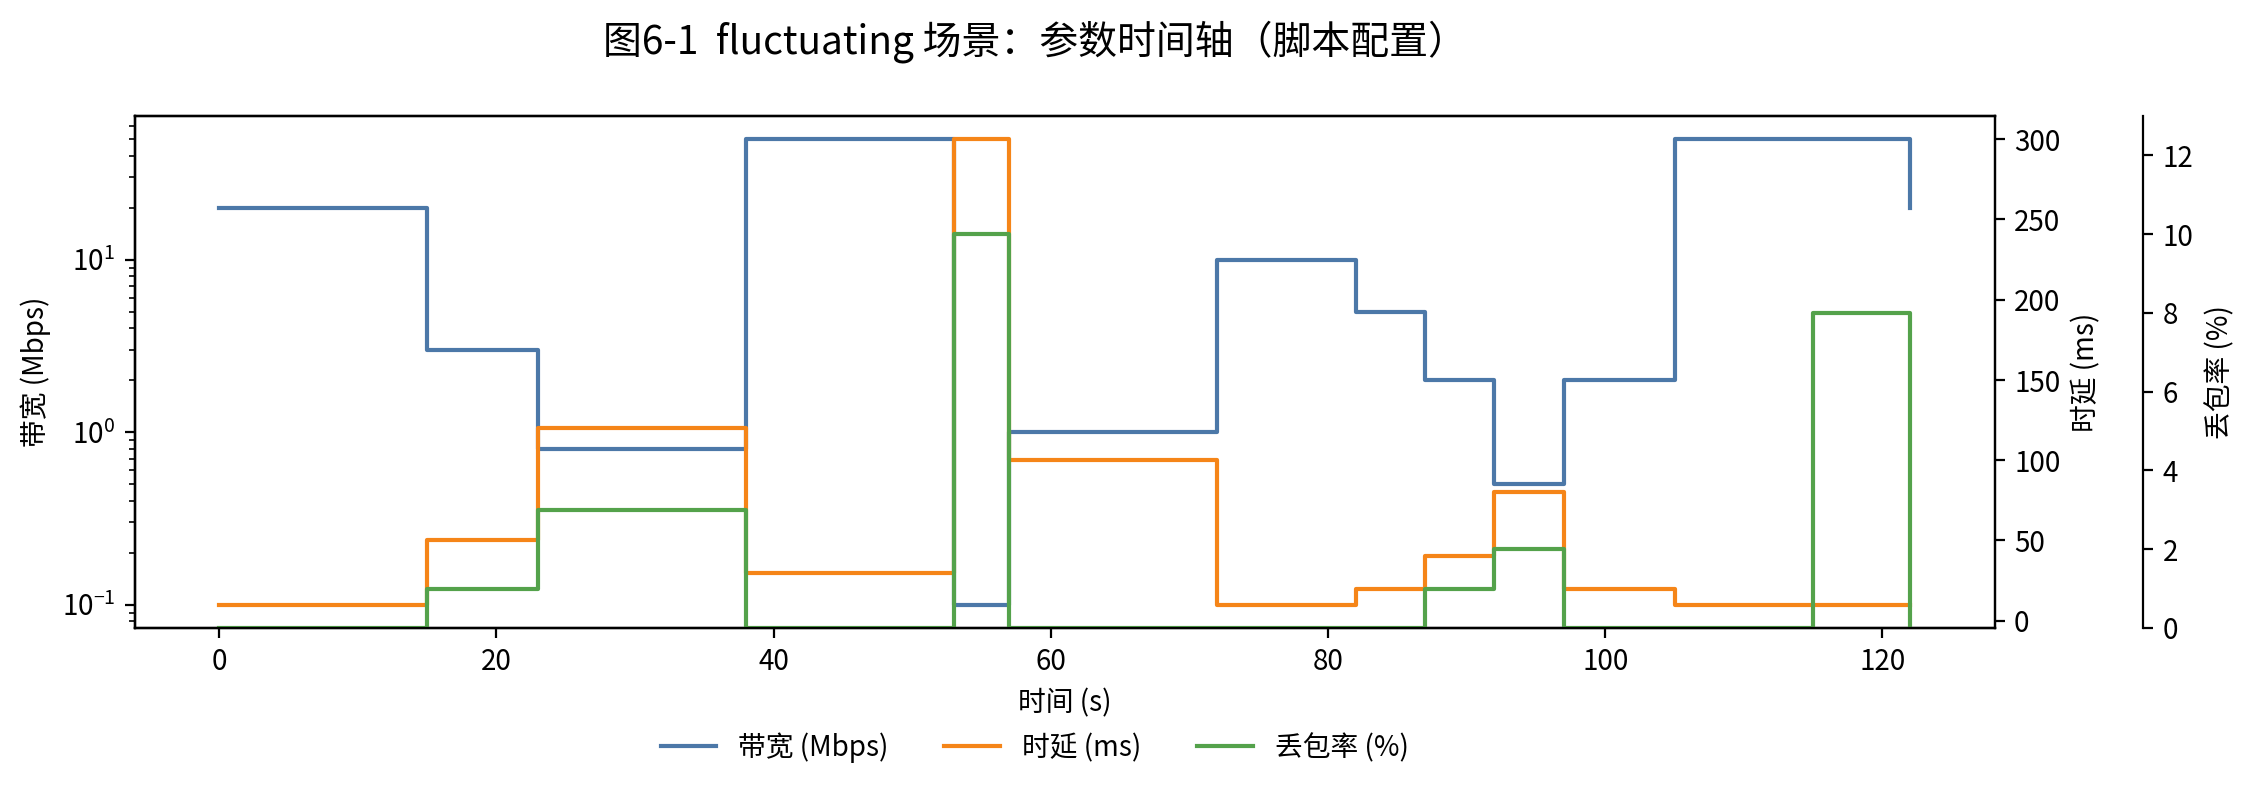
\includegraphics[width=0.95\textwidth]{figures/chapter6/fluctuating_paramters.png}
    \caption{\texttt{fluctuating} 场景：参数时间轴（脚本配置）}
    \label{fig:fluctuating-parameters}
\end{figure}

\section{A/B 测试流程与数据采集}

A/B 测试链路在 Node 服务端启动独立端口（默认 3001），两台终端设备打开 \texttt{ab\_test.html} 并在同一局域网内建立 WebRTC P2P 连接；每次实验固定使用同一段本地视频文件生成发送流，以减少内容复杂度差异对编码码率的影响。分组方式上，本研究采用“对照组 GCC / 实验组 RL + 限速 / 随机 50/50”三种模式中的随机模式作为默认配置，使每次连接在会话开始阶段随机分配到 GCC 或 RL 组，从而在多次重复试验中降低人为选择偏差。

\begin{figure}[htbp]
    \centering
    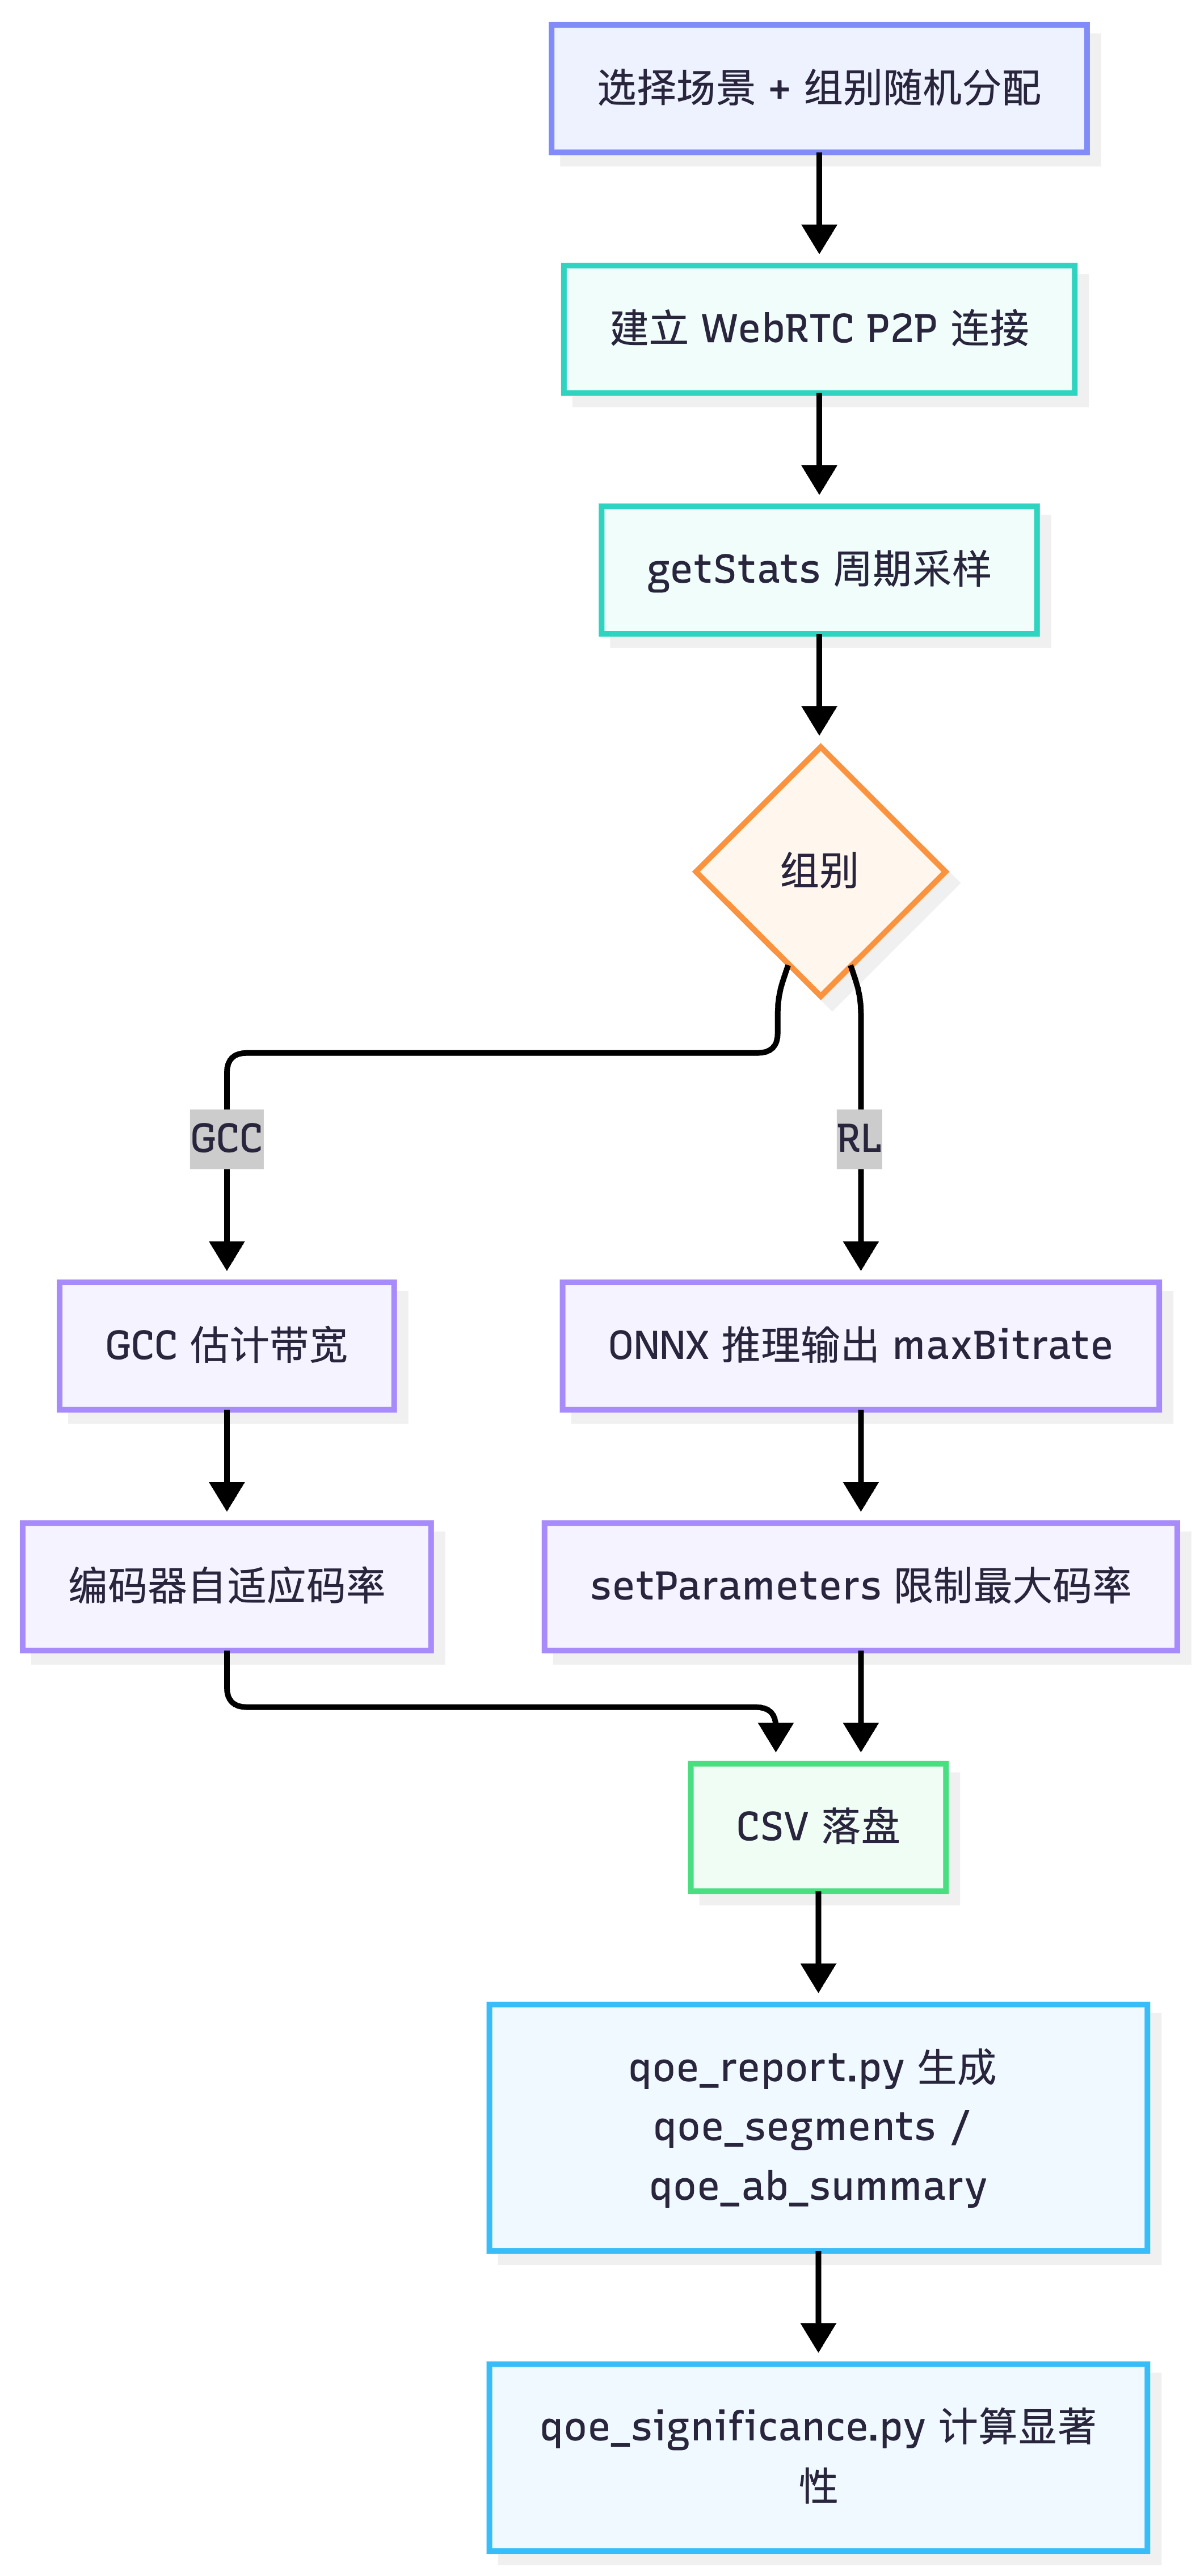
\includegraphics[width=0.95\textwidth]{figures/chapter6/ab_test_procedure.png}
    \caption{A/B 测试流程图}
    \label{fig:ab-test-procedure}
\end{figure}

采样与记录方面，前端通过 \texttt{getStats()} 周期性获取 WebRTC 关键统计量，并以 CSV 形式上报到服务端落盘；当采用浏览器本地 ONNX 推理时，数据写入 \texttt{ab\_test\_onnx\_csv/webrtc\_abtest\_traces\_\{scenario\}\_\{traceStartTs\}.csv}。基于现有实验数据，所有场景均采集到对照组与实验组各 10 条 trace，每条 trace 由两端设备分别生成一个 client 片段，因此每个 \texttt{(scenario, ab\_group)} 对应 20 个 client 统计片段；单条 trace 的有效持续时间约为 249.5 s，该时长略小于脚本设定的场景驻留时间（300 s），主要源于连接建立、媒体轨初始化与前后端同步过程带来的有效窗口裁剪。

\section{QoE 指标体系与计算方法}

为了使不同拥塞控制策略在真实链路中的表现能够被统一、可复现地量化，本研究基于 \texttt{tools/qoe\_report.py} 实现 QoE 评估脚本，对 A/B 测试采集到的 CSV 轨迹进行两级聚合：首先以“单个 CSV 文件 + 单个 clientId”为单位计算每段会话片段的 QoE 指标（输出 \texttt{output/qoe\_segments.csv}）；随后按 \texttt{(scenario, ab\_group)} 对片段指标取均值，形成场景级 A/B 汇总表（输出 \texttt{output/qoe\_ab\_summary.csv}）。

指标定义与计算口径如下。

\begin{enumerate}
    \item \textbf{吞吐（recv\_bps\_mean）}：片段内接收端吞吐 \texttt{recv\_bps} 的均值，用于衡量有效媒体接收速率。
    \item \textbf{时延（rtt\_ms\_p95）}：RTT 的 95 分位值，用于度量尾部时延；相比均值指标，P95 能更敏感地反映排队与抖动带来的交互劣化。
    \item \textbf{抖动（jitter\_ms\_p95）}：抖动的 95 分位值，用于刻画短时不稳定引发的播放风险。
    \item \textbf{丢包（loss\_rate\_mean）}：丢包率均值，反映链路可靠性与编码重传/冗余的潜在成本。
    \item \textbf{动作平滑性（cap\_delta\_bps\_mean）}：对“有效发送上限 cap”做一阶差分的绝对值均值，刻画码率上限的变化幅度。
\end{enumerate}

其中 cap 表示编码器实际生效的发送上限，本文在统计中以 \texttt{estimated\_bw\_bps} 作为 cap：在 RL 组中，策略通过 \texttt{RTCRtpSender.setParameters()} 只能限制最大码率，因此 \texttt{policy\_max\_bitrate\_bps} 反映的是策略给出的 \texttt{maxBitrate} 上限；当该上限大于 GCC 当前估计带宽 \texttt{gcc\_estimated\_bw\_bps} 时，编码器实际可用带宽仍受 GCC 估计约束，此时最终生效的发送上限将体现在 \texttt{estimated\_bw\_bps}（可理解为 \texttt{min(policy\_max\_bitrate\_bps, gcc\_estimated\_bw\_bps)}）。在 GCC 组中，\texttt{estimated\_bw\_bps} 通常与 \texttt{gcc\_estimated\_bw\_bps} 保持一致。为保证“动作平滑性”评价与真实生效控制量一致，本文统一使用 \texttt{estimated\_bw\_bps} 计算 cap\_delta，并保留 \texttt{policy\_max\_bitrate\_bps} 与 \texttt{gcc\_estimated\_bw\_bps} 用于诊断策略限速与 GCC 约束的相对关系。

综合 QoE 分数采用可复现的代理函数：

$$
\mathrm{QoE} = \log\left(1 + \frac{\mathrm{recv\_bps}}{10^6}\right) - \frac{\mathrm{rtt\_ms}}{1000} - \mathrm{loss\_rate} - 0.1 \cdot \frac{|\mathrm{cap}_t - \mathrm{cap}_{t-1}|}{10^6}
$$

该形式与第四章奖励函数保持一致，其设计逻辑是：使用对数函数描述吞吐收益的边际递减特性，同时对时延、丢包与码率震荡施加线性惩罚，从而使评价更接近实时视频通话对“稳定交互”的偏好。

\section{结果与分析}

\subsection{场景级 A/B 汇总}

本节显著性检验以 trace 为单位进行双侧置换检验；文中 p 值均为 BH 方法校正后的结果。

基于 \texttt{output/qoe\_ab\_summary.csv} 的汇总结果，RL 策略在多数弱网场景中呈现出一致的行为特征：吞吐略有降低，但 RTT 尾部、丢包率与动作波动显著下降，从而使综合 QoE 在高时延、低带宽、极端弱网等场景获得正向增益；在 baseline、dsl 与 fluctuating 等“带宽较充足或恢复阶段较快”的场景中，RL 策略存在一定的带宽利用不足，导致综合 QoE 略低于 GCC。

图 6-3 关键 QoE 指标分布对比（按场景）：

\begin{figure}[htbp]
    \centering
    \begin{minipage}{0.32\textwidth}
        \centering
        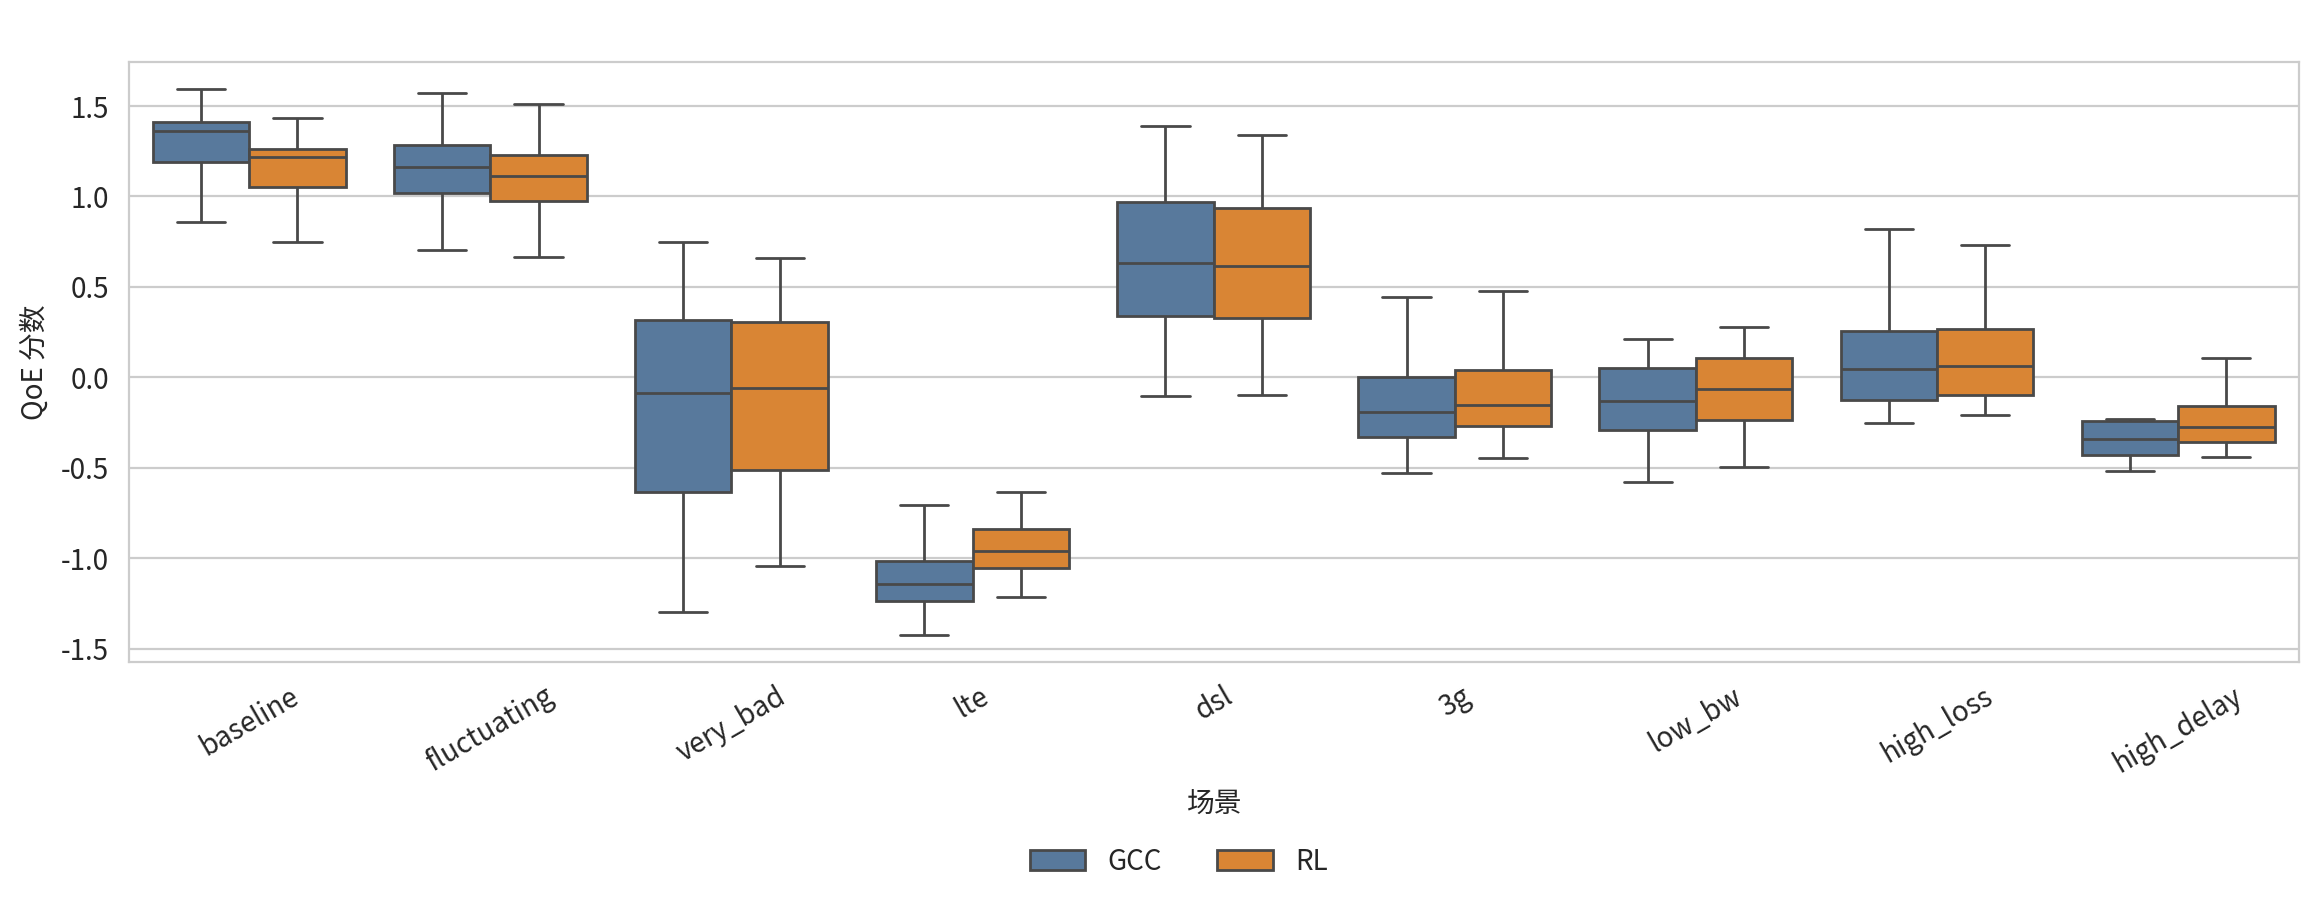
\includegraphics[width=\textwidth]{figures/chapter6/qoe_score.png}
        \caption{QoE 分数分布（按场景）}
        \label{fig:qoe-score}
    \end{minipage}\hfill
    \begin{minipage}{0.32\textwidth}
        \centering
        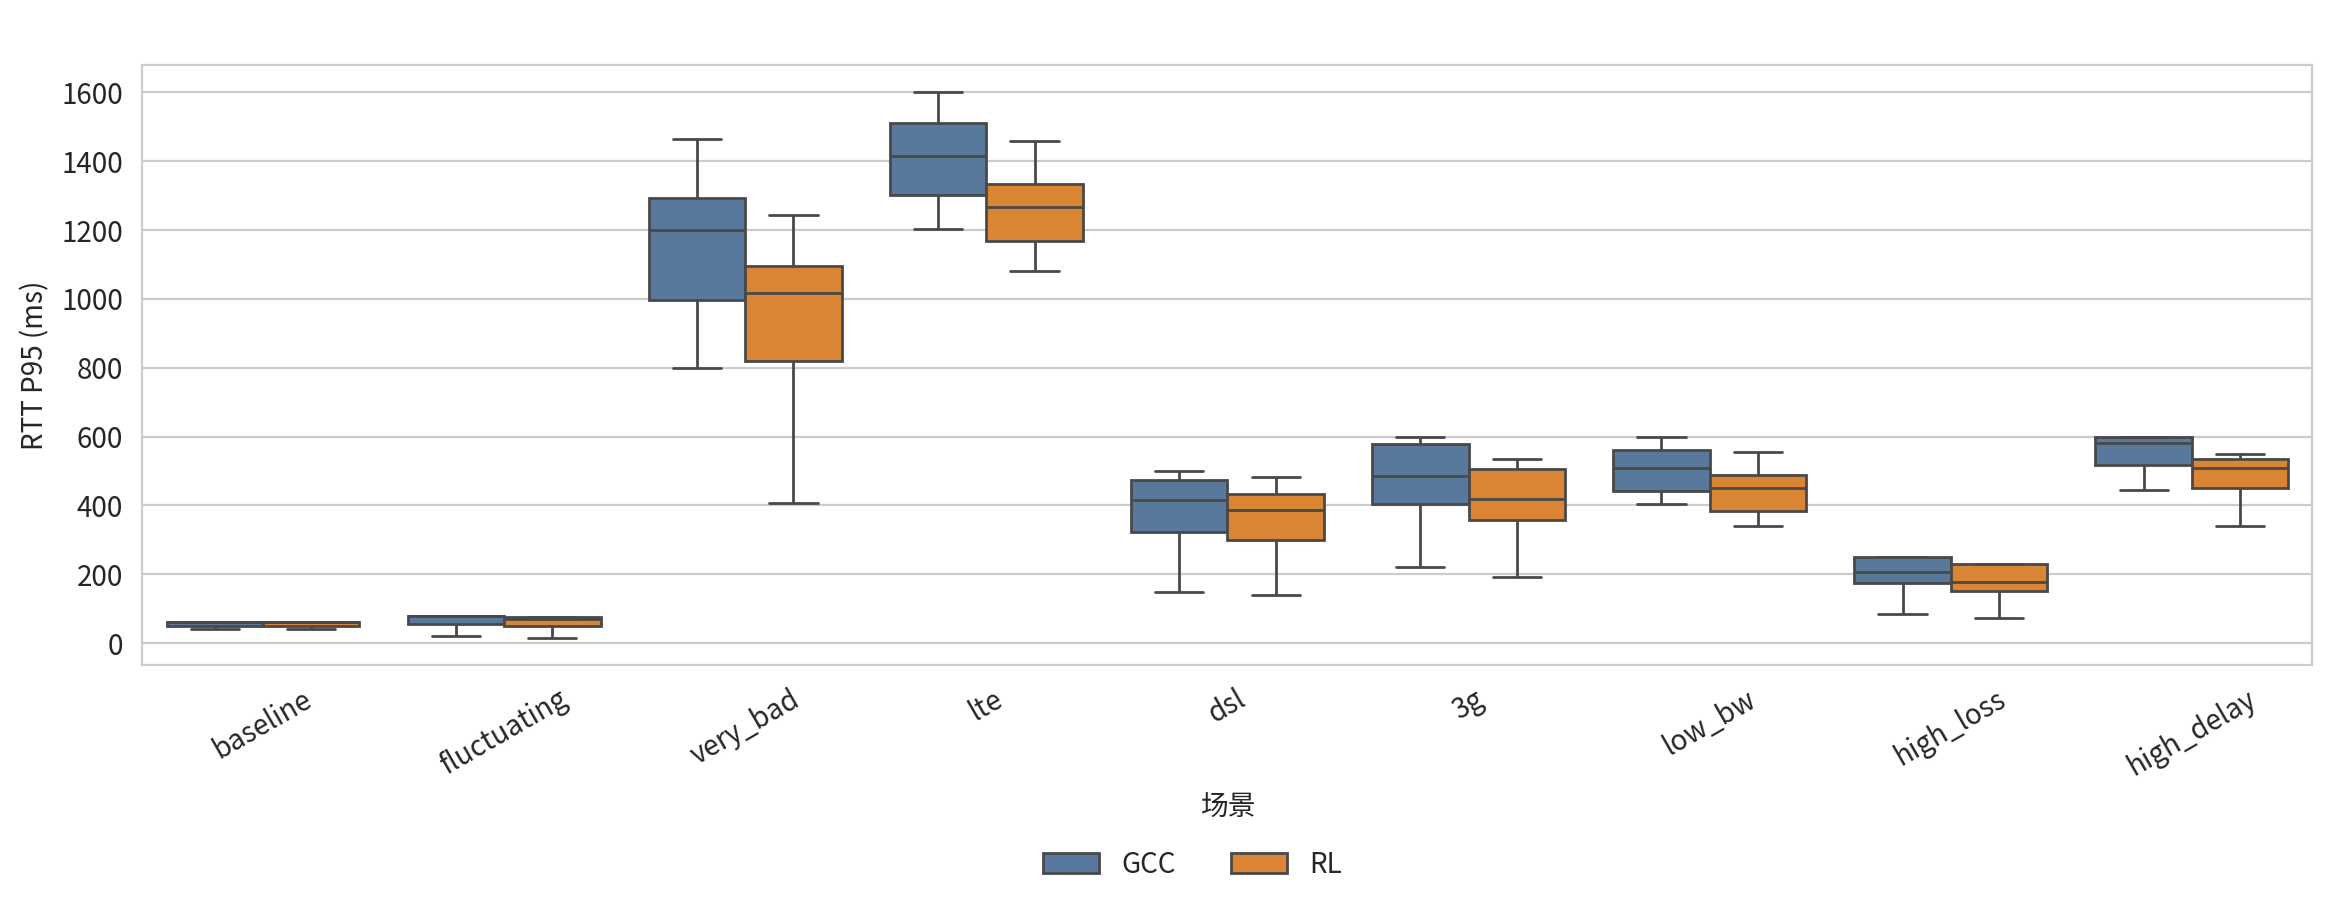
\includegraphics[width=\textwidth]{figures/chapter6/rtt_p95.png}
        \caption{RTT P95 分布（按场景）}
        \label{fig:rtt-p95}
    \end{minipage}\hfill
    \begin{minipage}{0.32\textwidth}
        \centering
        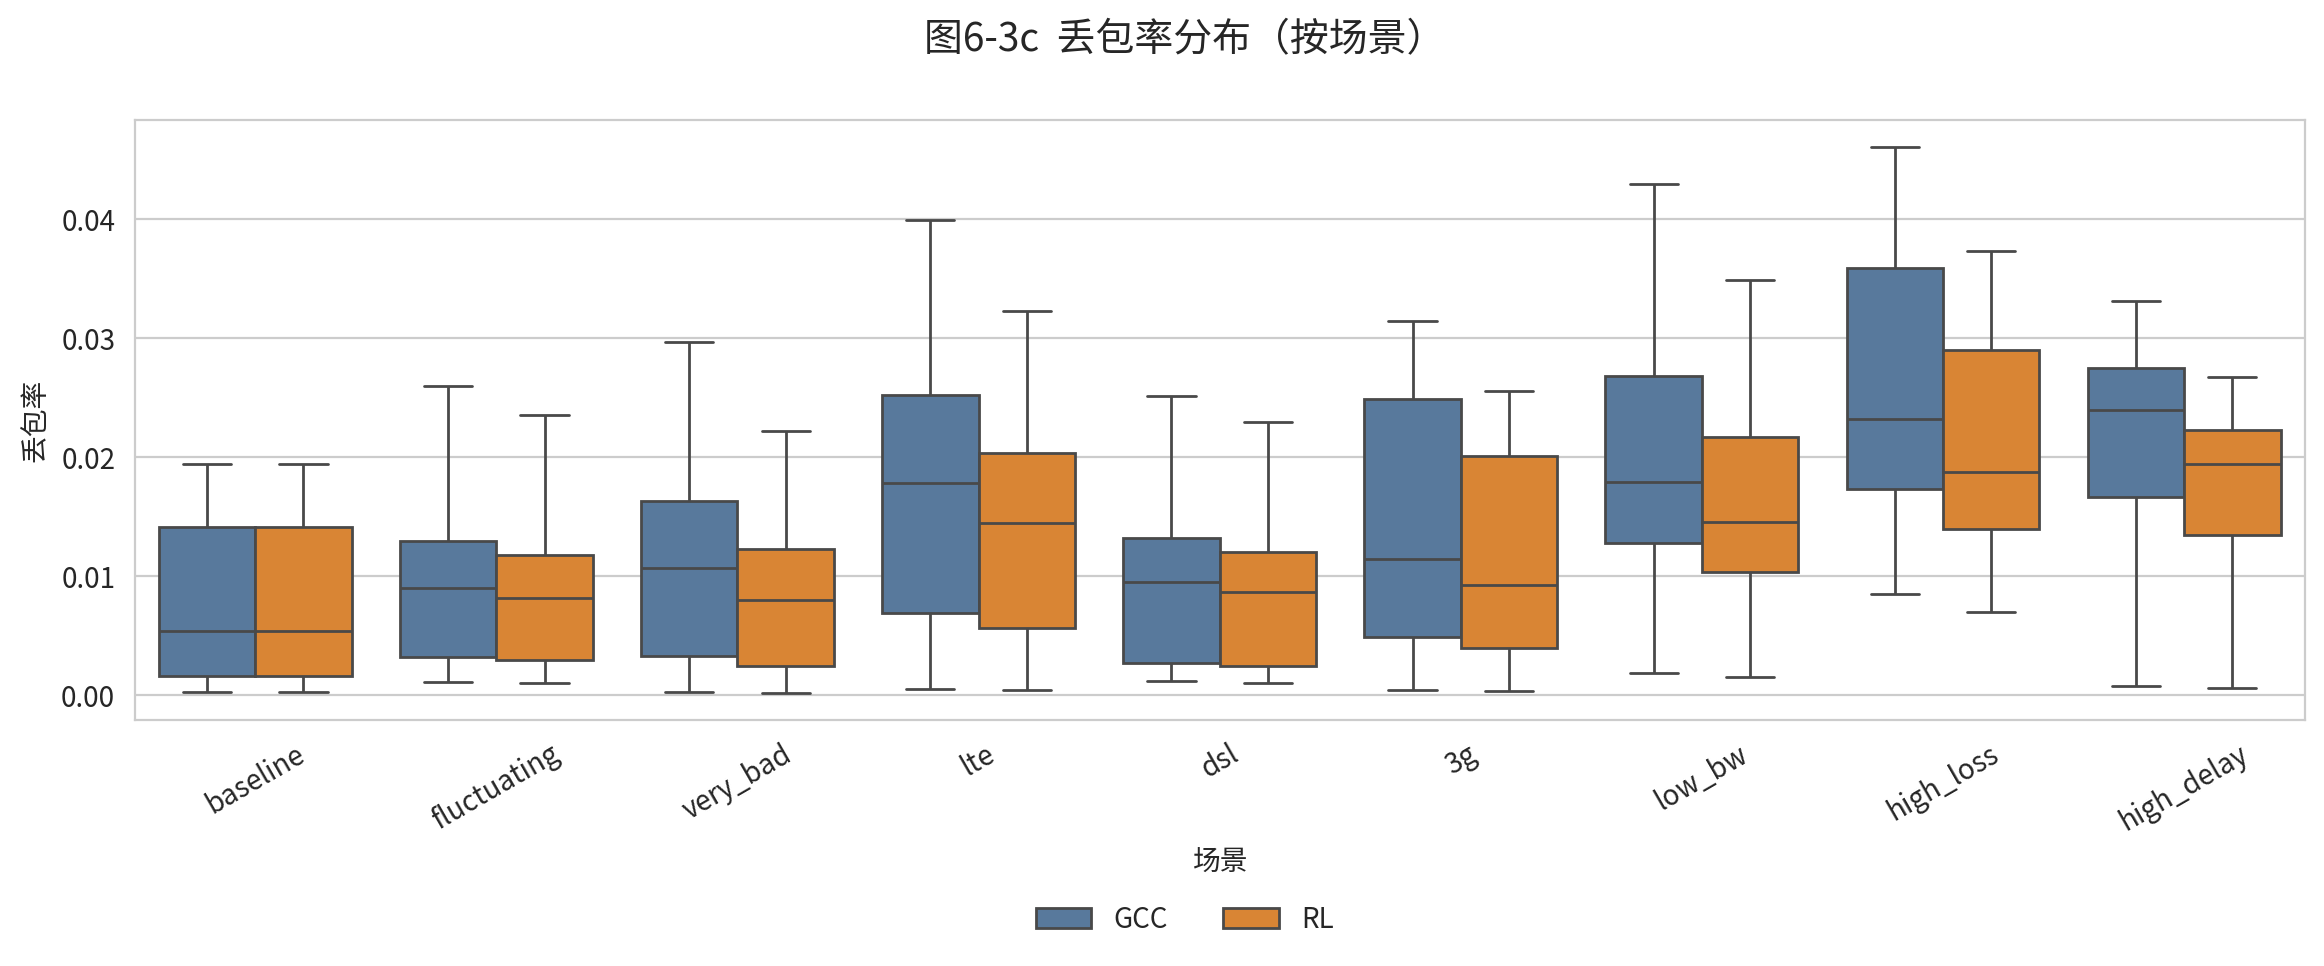
\includegraphics[width=\textwidth]{figures/chapter6/loss_rate.png}
        \caption{丢包率分布（按场景）}
        \label{fig:loss-rate}
    \end{minipage}
\end{figure}

\begin{figure}[htbp]
    \centering
    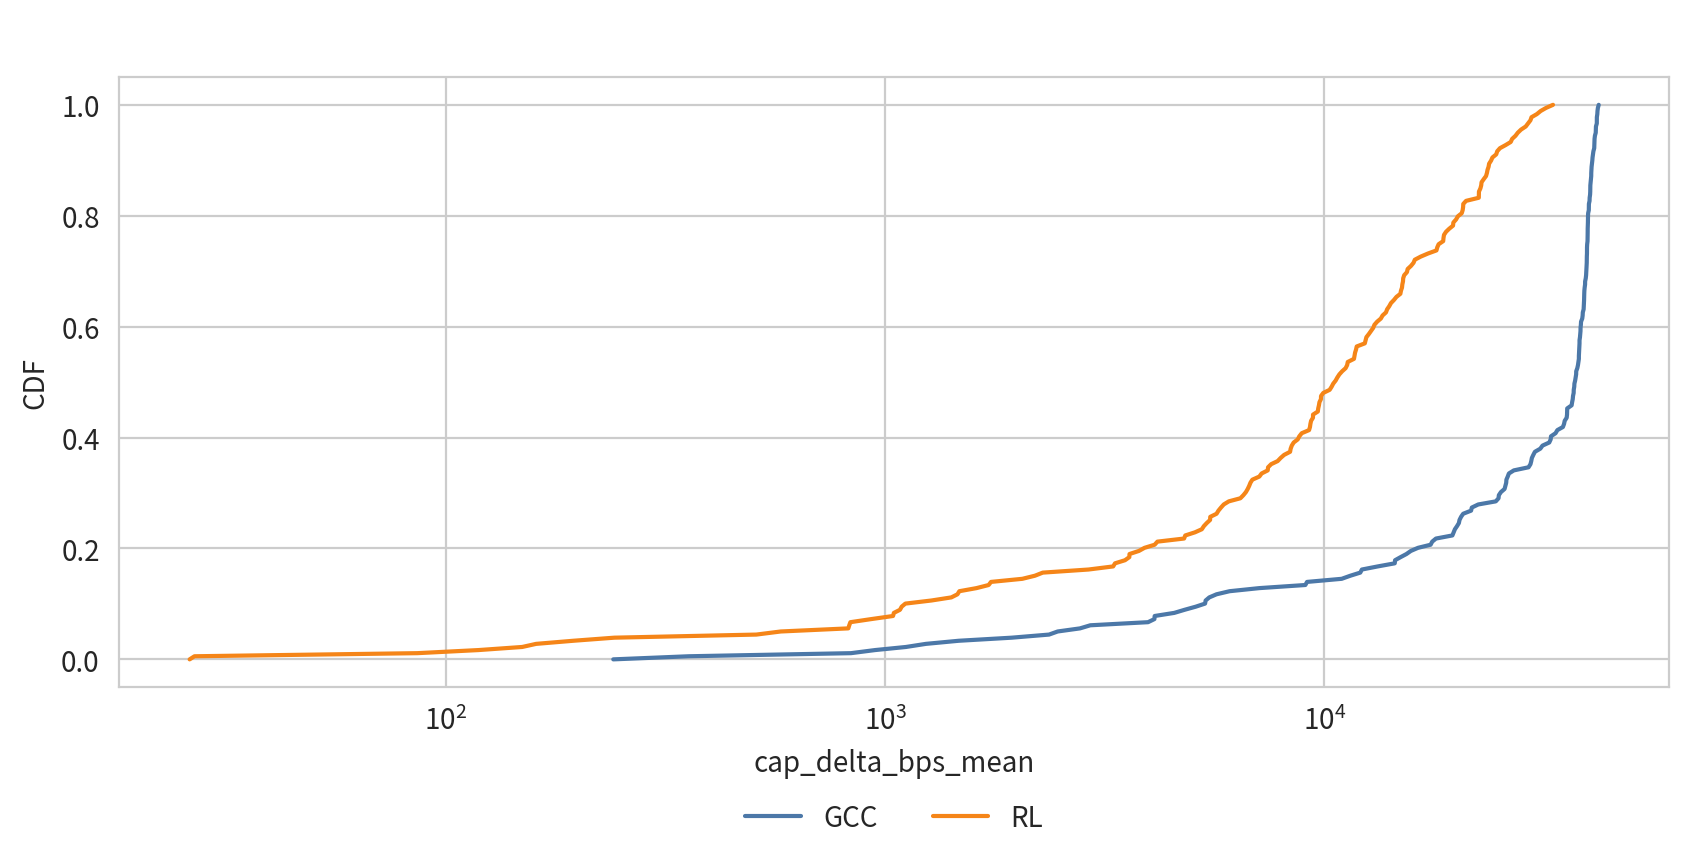
\includegraphics[width=0.9\textwidth]{figures/chapter6/cap.png}
    \caption{cap\_delta 分布 CDF（全场景合并）}
    \label{fig:cap-delta-cdf}
\end{figure}

\begin{figure}[htbp]
    \centering
    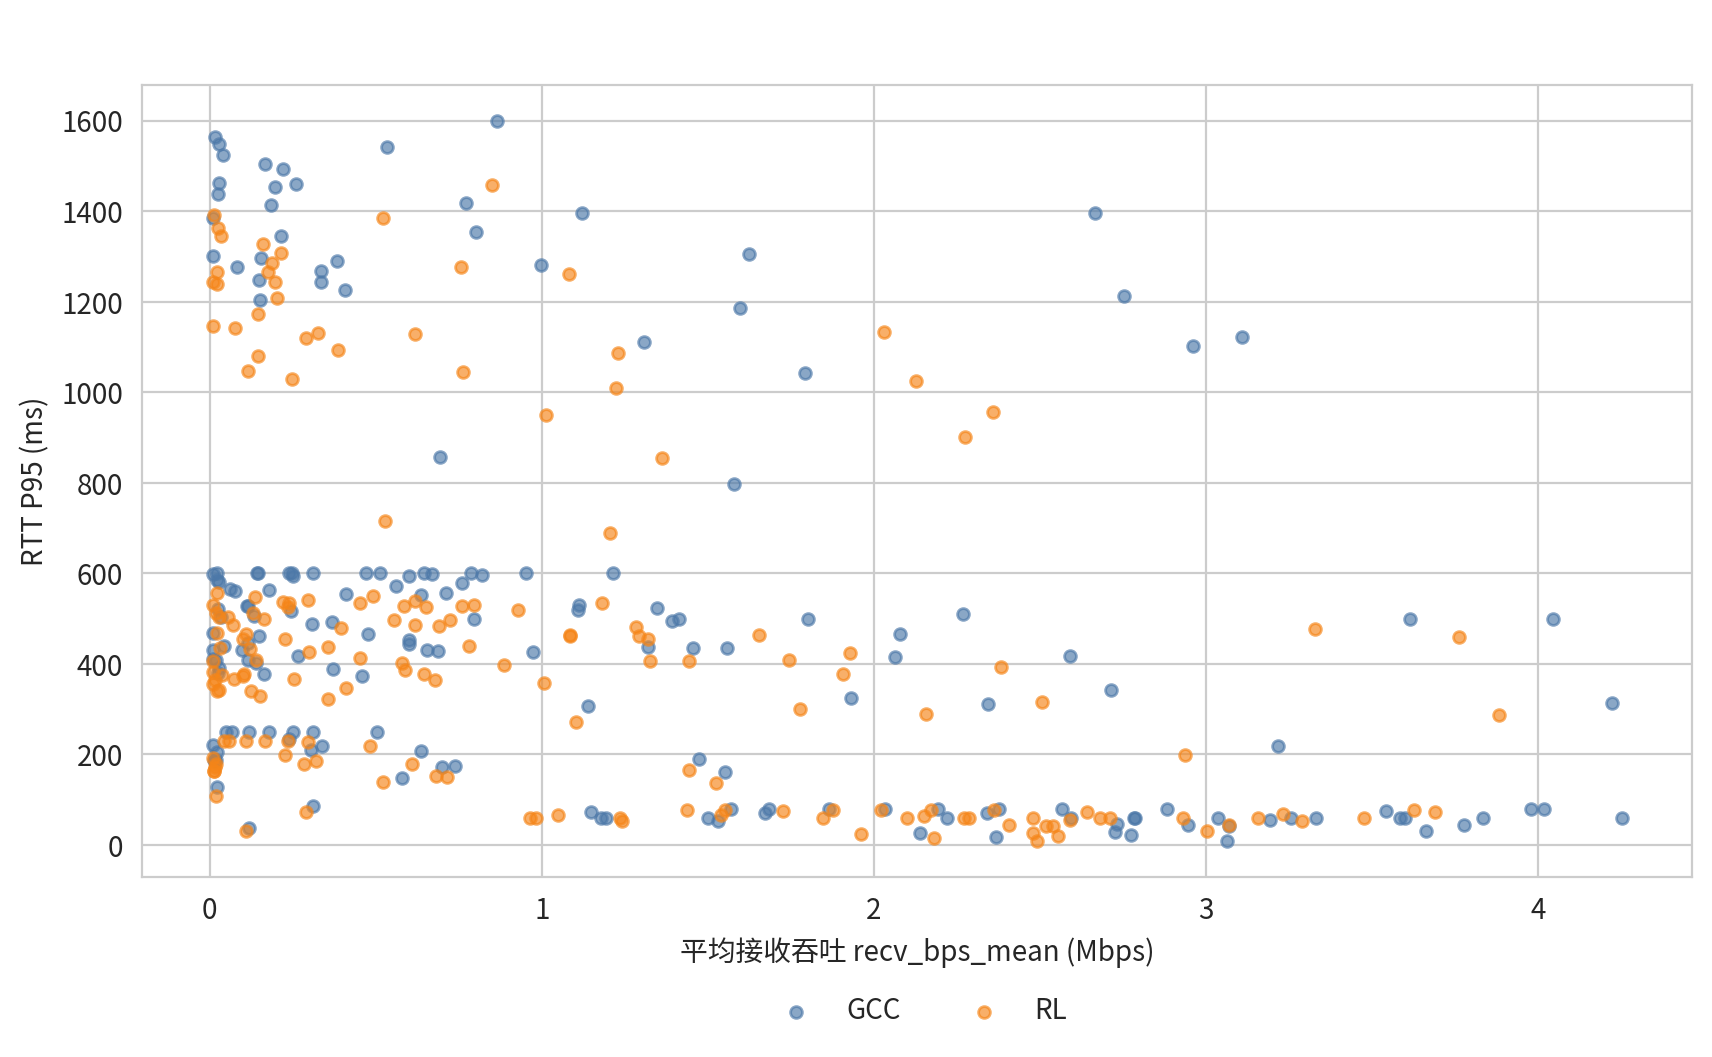
\includegraphics[width=0.9\textwidth]{figures/chapter6/throughtput_delay_tradeoff.png}
    \caption{吞吐-时延权衡散点图（每个 client 片段）}
    \label{fig:throughput-delay-tradeoff}
\end{figure}

为便于展示主要趋势，表 6-1 给出了各场景下 RL 相对于 GCC 的关键指标变化（百分比为相对 GCC 的变化率；QoE 以绝对差值表示）。

\begin{table}[htbp]
    \centering
    \small
    \begin{tabular}{|l|c|c|c|c|c|}
        \hline
        场景 & 吞吐变化 & RTT P95 变化 & 丢包率变化 & cap\_delta 变化 & QoE 差值（RL--GCC） \\
        \hline
        baseline & -18.19\% & 0.00\% & 0.00\% & -42.64\% & -0.137 \\
        3g & -3.65\% & -12.42\% & -19.10\% & -73.13\% & +0.054 \\
        dsl & -8.00\% & -7.05\% & -9.02\% & -50.07\% & -0.019 \\
        lte & -3.57\% & -10.82\% & -19.02\% & -73.36\% & +0.189 \\
        low\_bw & -3.17\% & -12.17\% & -19.02\% & -72.77\% & +0.062 \\
        high\_delay & -3.64\% & -11.81\% & -18.97\% & -70.59\% & +0.067 \\
        high\_loss & -3.71\% & -11.68\% & -19.01\% & -70.81\% & +0.018 \\
        fluctuating & -8.27\% & -6.42\% & -9.07\% & -46.06\% & -0.052 \\
        very\_bad & -23.55\% & -16.25\% & -25.14\% & -59.97\% & +0.055 \\
        \hline
    \end{tabular}
    \caption{各场景下 RL 相对于 GCC 的关键指标变化}
    \label{tab:ab-delta-summary}
\end{table}

从表 6-1 可以得到三点关键观察。

第一，\textbf{动作平滑性（cap\_delta）在所有场景中均显著下降}，下降幅度落在 42\%--73\% 区间，表明离线强化学习策略在动作序列上倾向于输出更稳定的带宽上限，能够有效抑制 GCC 在弱网反馈噪声下常见的“快速升降—再回退”的振荡行为。基于 \texttt{output/qoe\_significance.csv} 的结果可发现，cap\_delta 在所有场景中均显著下降（p$\le$0.0012），说明该收益具有较强统计稳健性。

第二，\textbf{RTT P95 与丢包率在多数弱网场景中同步降低}。在 3g、lte、low\_bw、high\_delay、very\_bad 等场景中，RTT P95 的下降约为 10\%--16\%，丢包率下降约为 18\%--25\%，反映 RL 策略更倾向于通过保守限速避免排队积压，使网络处于“低排队、低重传压力”的工作点。RTT P95 在 high\_delay、low\_bw 与 lte 场景下降显著（p 分别为 0.028、0.037、0.026），very\_bad 场景接近显著（p=0.051）。丢包率虽呈下降趋势，但在当前样本规模下未达显著（各场景 p$>$0.3）。

第三，\textbf{吞吐在多数场景中略有下降，但在 baseline 与 very\_bad 场景存在明显的带宽利用不足}。baseline 场景中 RTT、丢包与抖动基本不变，RL 仍降低了 18\% 的平均吞吐并使 QoE 下降 0.137，说明当前奖励权重与策略学习到的保守偏置可能导致“高质量网络下的过度限速”；very\_bad 场景中，RL 将 RTT P95 与丢包率分别降低 16\% 与 25\%，但吞吐下降 24\%，使综合 QoE 仅获得有限提升，表明在极端弱网下，吞吐收益项与惩罚项的权衡仍需进一步精细化。

\subsection{代表性场景讨论}

\begin{enumerate}
    \item \textbf{LTE 场景：弱网收益最明显。} 在 LTE 场景中，RL 将 RTT P95 从 1410 ms 降至 1258 ms，同时将 cap\_delta 降低 73\%，综合 QoE 从 -1.115 提升至 -0.926（差值 +0.189），QoE 提升接近显著（p=0.051）。综合 RTT 与 cap\_delta 的显著改善，可认为 RL 在该类“中等带宽 + 较高时延”场景具备较明确的稳定性收益。
    \item \textbf{high\_delay / low\_bw 场景：以吞吐换取交互稳定性。} 这两类场景共同特点是“瓶颈由时延或带宽主导”，RL 在吞吐仅下降约 3\% 的前提下，将 RTT P95 降低约 12\%、丢包率降低约 19\%，并显著降低动作波动，从而使 QoE 分数分别提升 +0.067 与 +0.062。该现象与奖励函数对时延与丢包的惩罚一致，说明策略确实学到了以交互稳定性为优先目标的控制偏好。
    \item \textbf{fluctuating 场景：动态恢复阶段的带宽利用不足。} fluctuating 场景在同一轨迹内包含“带宽断崖、短时恢复与再次拥塞”等多阶段变化，RL 虽然降低了 RTT 与丢包并减少动作波动，但吞吐下降 8\% 且 QoE 略低于 GCC（-0.052）。其潜在原因在于：离线训练数据主要来源于 GCC 行为轨迹，且策略更新采用优势加权行为克隆，策略对“快速恢复阶段的激进探测”学习不足；同时，为保证部署安全性，推理管线中引入 EMA 平滑与单步限幅，进一步降低了策略对带宽骤增时的响应速度。
\end{enumerate}

\section{本文方案的优势与局限}

\subsection{优势}

\begin{enumerate}
    \item \textbf{训练风险低且具备可部署闭环。} 本研究采用离线强化学习直接利用 GCC 历史轨迹训练策略，避免在线探索对真实通话造成的质量扰动，并通过 ONNX 导出与浏览器本地推理将策略无缝嵌入 WebRTC 控制回路，形成“采集—训练—部署—A/B 验证”的可重复工程闭环。
    \item \textbf{在弱网场景获得更稳定的控制行为。} A/B 结果表明 RL 在所有场景下显著降低 cap\_delta，说明策略输出更加平滑，有助于减少编码器频繁调参带来的画面质量抖动，也降低了“过冲—回退”型振荡对排队时延与丢包的放大效应。
    \item \textbf{对多类扰动具有一致的降时延与降丢包趋势。} 在 3g、lte、low\_bw、high\_delay 与 very\_bad 等场景中，RL 同时降低 RTT P95 与丢包率，体现出对排队积压的主动抑制能力；该趋势与离线奖励函数的设计目标一致，证明本文的状态特征选择与奖励构造能够在真实系统中传递有效优化信号。
\end{enumerate}

\subsection{局限}

\begin{enumerate}
    \item \textbf{QoE 评价函数仍是代理指标。} 本文采用的 QoE 分数由吞吐、RTT、丢包与动作波动构成，具有可复现与易实现的优点，但尚未直接覆盖视频主观体验中的关键因素，例如帧率、分辨率变化、卡顿/冻结时长、解码丢帧等，因此其与真实 MOS 的映射关系仍需进一步研究。
    \item \textbf{样本规模与实验维度有限。} 现有 A/B 数据在每个场景下仅包含 10 条 trace，且设备类型、浏览器版本、编码参数与视频内容形式相对固定，统计显著性在部分指标上不够稳定；在更大规模、更异构终端与更复杂网络环境下的泛化表现仍有待补充验证。
    \item \textbf{对高质量网络存在保守估计。} baseline 场景中 RL 的吞吐显著低于 GCC 且 RTT/丢包无明显改善，说明在当前奖励权重与训练数据分布下，策略可能学习到过度保守的限速倾向；后续可考虑引入更强的“带宽利用率”约束、对不同场景自适应调权，或在离线训练阶段加入更丰富的高带宽样本以缓解偏置。
    \item \textbf{离线强化学习的分布外风险仍然存在。} 尽管 IQL 在工程上更稳定，但策略本质上仍从行为策略数据中外推决策边界；当真实网络状态出现训练数据未覆盖的组合模式（例如突发长时间的纯丢包、时延估计异常等），策略可能产生不可预期动作，因此部署侧仍需保留 OOD 检测、动作限幅与回退机制。
\end{enumerate}

\subsection{适用部署环境与指标关注偏好}

基于前述实验结果，本文所提出的离线强化学习拥塞控制模型在特定网络环境与业务目标下展现出明确的适用性。总体而言，该模型更适合部署于无线接入与各类受限网络环境，尤其是在业务更关注交互实时性与稳定性的场景中。

具体到网络环境，模型在 \texttt{3g}、\texttt{lte}、\texttt{low\_bw}、\texttt{high\_delay} 及 \texttt{very\_bad} 等模拟真实弱网条件下的表现尤为突出。在这些场景中，链路本身存在带宽瓶颈、高延迟或随机丢包等问题，实验结果一致表明，IQL 策略通过更为保守和平滑的码率调节，能够有效抑制网络排队积压，从而在降低 RTT 高分位值（RTT P95）与平均丢包率方面取得相较于 GCC 的稳定收益。然而，在 \texttt{fluctuating} 这类网络容量能够快速恢复的场景中，模型的保守倾向使其无法充分利用链路带宽，导致吞吐量下降。这表明，当网络环境需要更激进的带宽探测以快速抢占可用资源时，当前模型并非最优选择。

从业务指标的关注偏好来看，当应用场景对交互的实时性与稳定性要求高于极致的峰值吞吐时，本模型具有显著优势。实验数据显示，模型在多数场景下以微小的吞吐量下降为代价，换取了 RTT、丢包率、抖动以及码率变化平滑性等多个维度的显著改善。这对于在线会议、云游戏、远程控制等对延迟和卡顿极其敏感的应用至关重要。反之，若业务场景以大文件传输或超高清视频点播为主，其核心目标是最大化带宽利用率与峰值画质，且能容忍一定程度的时延波动与码率振荡，那么直接采用当前模型需谨慎评估。在此类场景下，可能需要通过调整奖励函数中各项指标的权重，或引入更多高带宽利用率的专家轨迹数据对模型进行再训练，以强化其带宽探索能力。

\section{本章小结}

本章基于真实 WebRTC 端到端平台，构建了覆盖九类典型网络条件的 A/B 测试评估流程，并以可复现的 QoE 指标体系对 GCC 与离线强化学习策略进行了系统比较。结果表明，离线强化学习策略能够在多数弱网场景中显著降低码率动作波动，并呈现出降低 RTT 尾部与丢包率的稳定趋势，从而在 LTE、低带宽与高时延等场景获得正向 QoE 收益；与此同时，策略在高质量网络与部分动态波动场景中存在带宽利用不足，提示后续需要在奖励权重、训练数据覆盖与安全约束之间进行进一步权衡与优化。
